Send notification is a feature that is not in the requirement documentation but was asked to be added in by our client. It allows him to send notifications to remind patience of their next follow up. 
The send notification use case unit tests failed because the schema could not be found, see figure bellow.
\newline 
\newline 
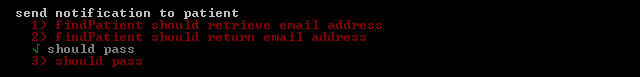
\includegraphics[width=350px]{./TestingDoc/Graphics/SendNotification}
\newline
\newline
Test failure causes
\newline
\newline
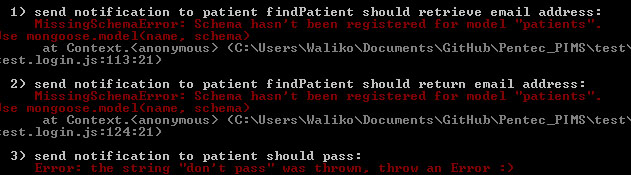
\includegraphics[width=350px]{./TestingDoc/Graphics/FailedTests}
\newline
\newline
The following pre and post conditions for the send notification must hold true.
		
\subsubsection*{Conditions}
The following pre and post conditions are defined for adding a new user.
	
\subsubsection*{Pre conditions}	
\begin{itemize}
		\item User must be logged in as administrator.
		\item Patient must exist in the system database.
		\item Patient must have an active email account.
\end{itemize}	

\subsubsection*{Post conditions}	
\begin{itemize}
		\item A notification informing patient about their next appointment is sent to the users email account. 
\end{itemize}	

Code snippets for send notification use case that looks for a patient email address in the database to send a notification to.	
\newline

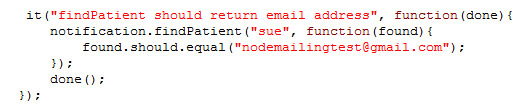
\includegraphics[width=350px]{./TestingDoc/Graphics/find}

\subsubsection*{Remark}
Since Send notification fails unit testing, the module needs to be revised and tested again.